\newpage
\addcontentsline{toc}{section}{Results}
\section*{Results}

\phantomsection

\addcontentsline{toc}{subsection}{Models Sensitivity to Unconstrained Hydraulic Parameters}
\subsection*{Models Sensitivity to Unconstrained Hydraulic Parameters}

\textbf{NOTE: Unconstrained parameter uncertainty figures are preliminary and although wet and dry years look the same, the numbers are different. However, they do generally fit my hypothesis and I am assuming that when I do my final runs the variance will increase because these are back of the envelope calculations.}

When considering model predictive variance attributed to hydraulic parameters before constraining parameter priors, ED-hydro does not show a clear improvement over ED2. Under both wet and dry conditions, ED2-hydro predictive variance attributed to hydraulic variables is higher for GPP, NPP and Soil Moisture. The only exception is the prediction of Transpiration, where the ED2-hydro predictive variance is lower. (This could change in the results and I should also note the actual units of these intervals of difference.) 

\addcontentsline{toc}{subsection}{Models Sensitivity to Constrained Hydraulic Parameters}
\subsection*{Models Sensitivity to Constrained Hydraulic Parameters} 

After completing the meta-analysis and constraining all nine hydraulic parameters, the results change significantly.  Under all scenarios ED2-hydro total predictive variance attributed to hydraulic traits was consistently less than the predictive uncertainly from the ED2 runs attributed to water conductance. Thus, ED2-hydro showed a clear and significant improvement over ED2. 

\begin{figure}[!h]
    \centering
    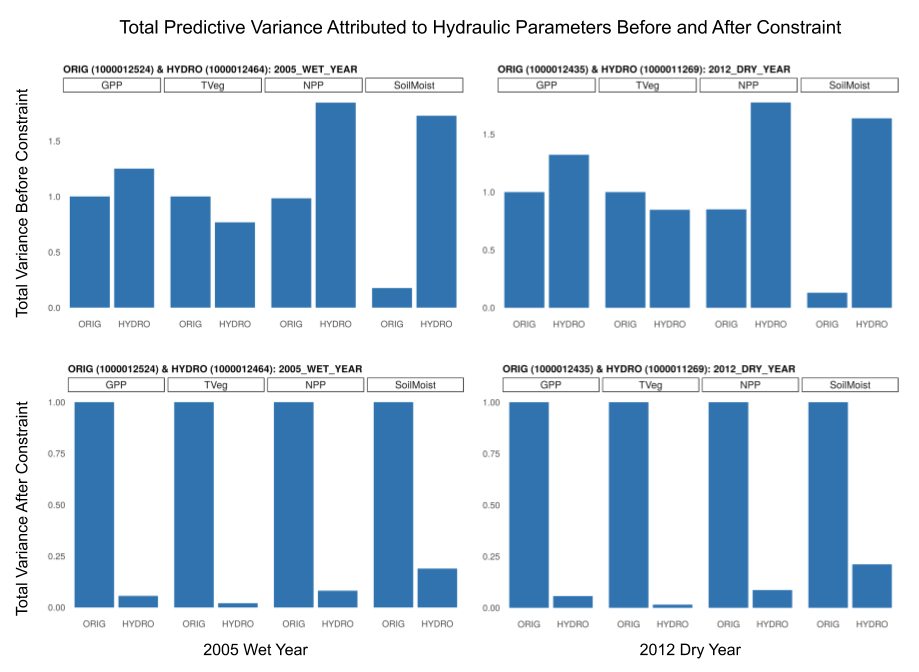
\includegraphics[width=.9\textwidth]{Hydro_Paper_LaTeX/Hydro_Paper_Figures/variance_before_after.png}
    \caption[Hydraulic variance]{Total variance attributed to hydraulic parameters before contraint and after constraint.
    
    \todoq{In this figure, would it be useful to partition the uncertainty in the ED-hydro bars out by trait (to emphasize the fact that the total variance is the sum of the contribution of multiple traits, where in the case of ED2, it is JUST water conductance?)}}
    \label{fig:constraint_var}
\end{figure}

%%%%%%%%%%%%%%%%%%%%%%%%%%%%%%%%%%%%%%%%%%%%%%%%%%%%%%%%%%%%%%%%%%%%%%%%%%%%%%
\addcontentsline{toc}{subsection}{Comparison of Total Predictive Uncertainty}
\subsection*{Comparison of Total Predictive Variance}

Although ED2-hydro showed a reduction in predictive uncertainty attributed  to hydraulic parameters in relation to ED2, this was not the case when comparing total predictive variance. Under water stress conditions, the structural differences in ED2-hydro not only resulted in increased sensitivity to hydraulic parameters, but also to non-hydraulics parameters associated with leaf and root biomass allocation. While it was possible to constrain priors for leaf biomass allocation parameter , data was not available to those for root biomass allocation.  Thus, for calculations of state variables such as soil moisture under water stress in which root growth plays an important role, uncertainty attributed to root biomass allocation dominated total predictive variance, resulting in a higher total predictive variance than ED2. In the case of NPP, GPP and Transpiration, ED2-hydro did not show significant changes in model sensitivity to non-hydraulic parameters between dry and wet years and thus total predictive variance remained lower than that of ED2. 

\begin{figure}[!h]
    \centering
    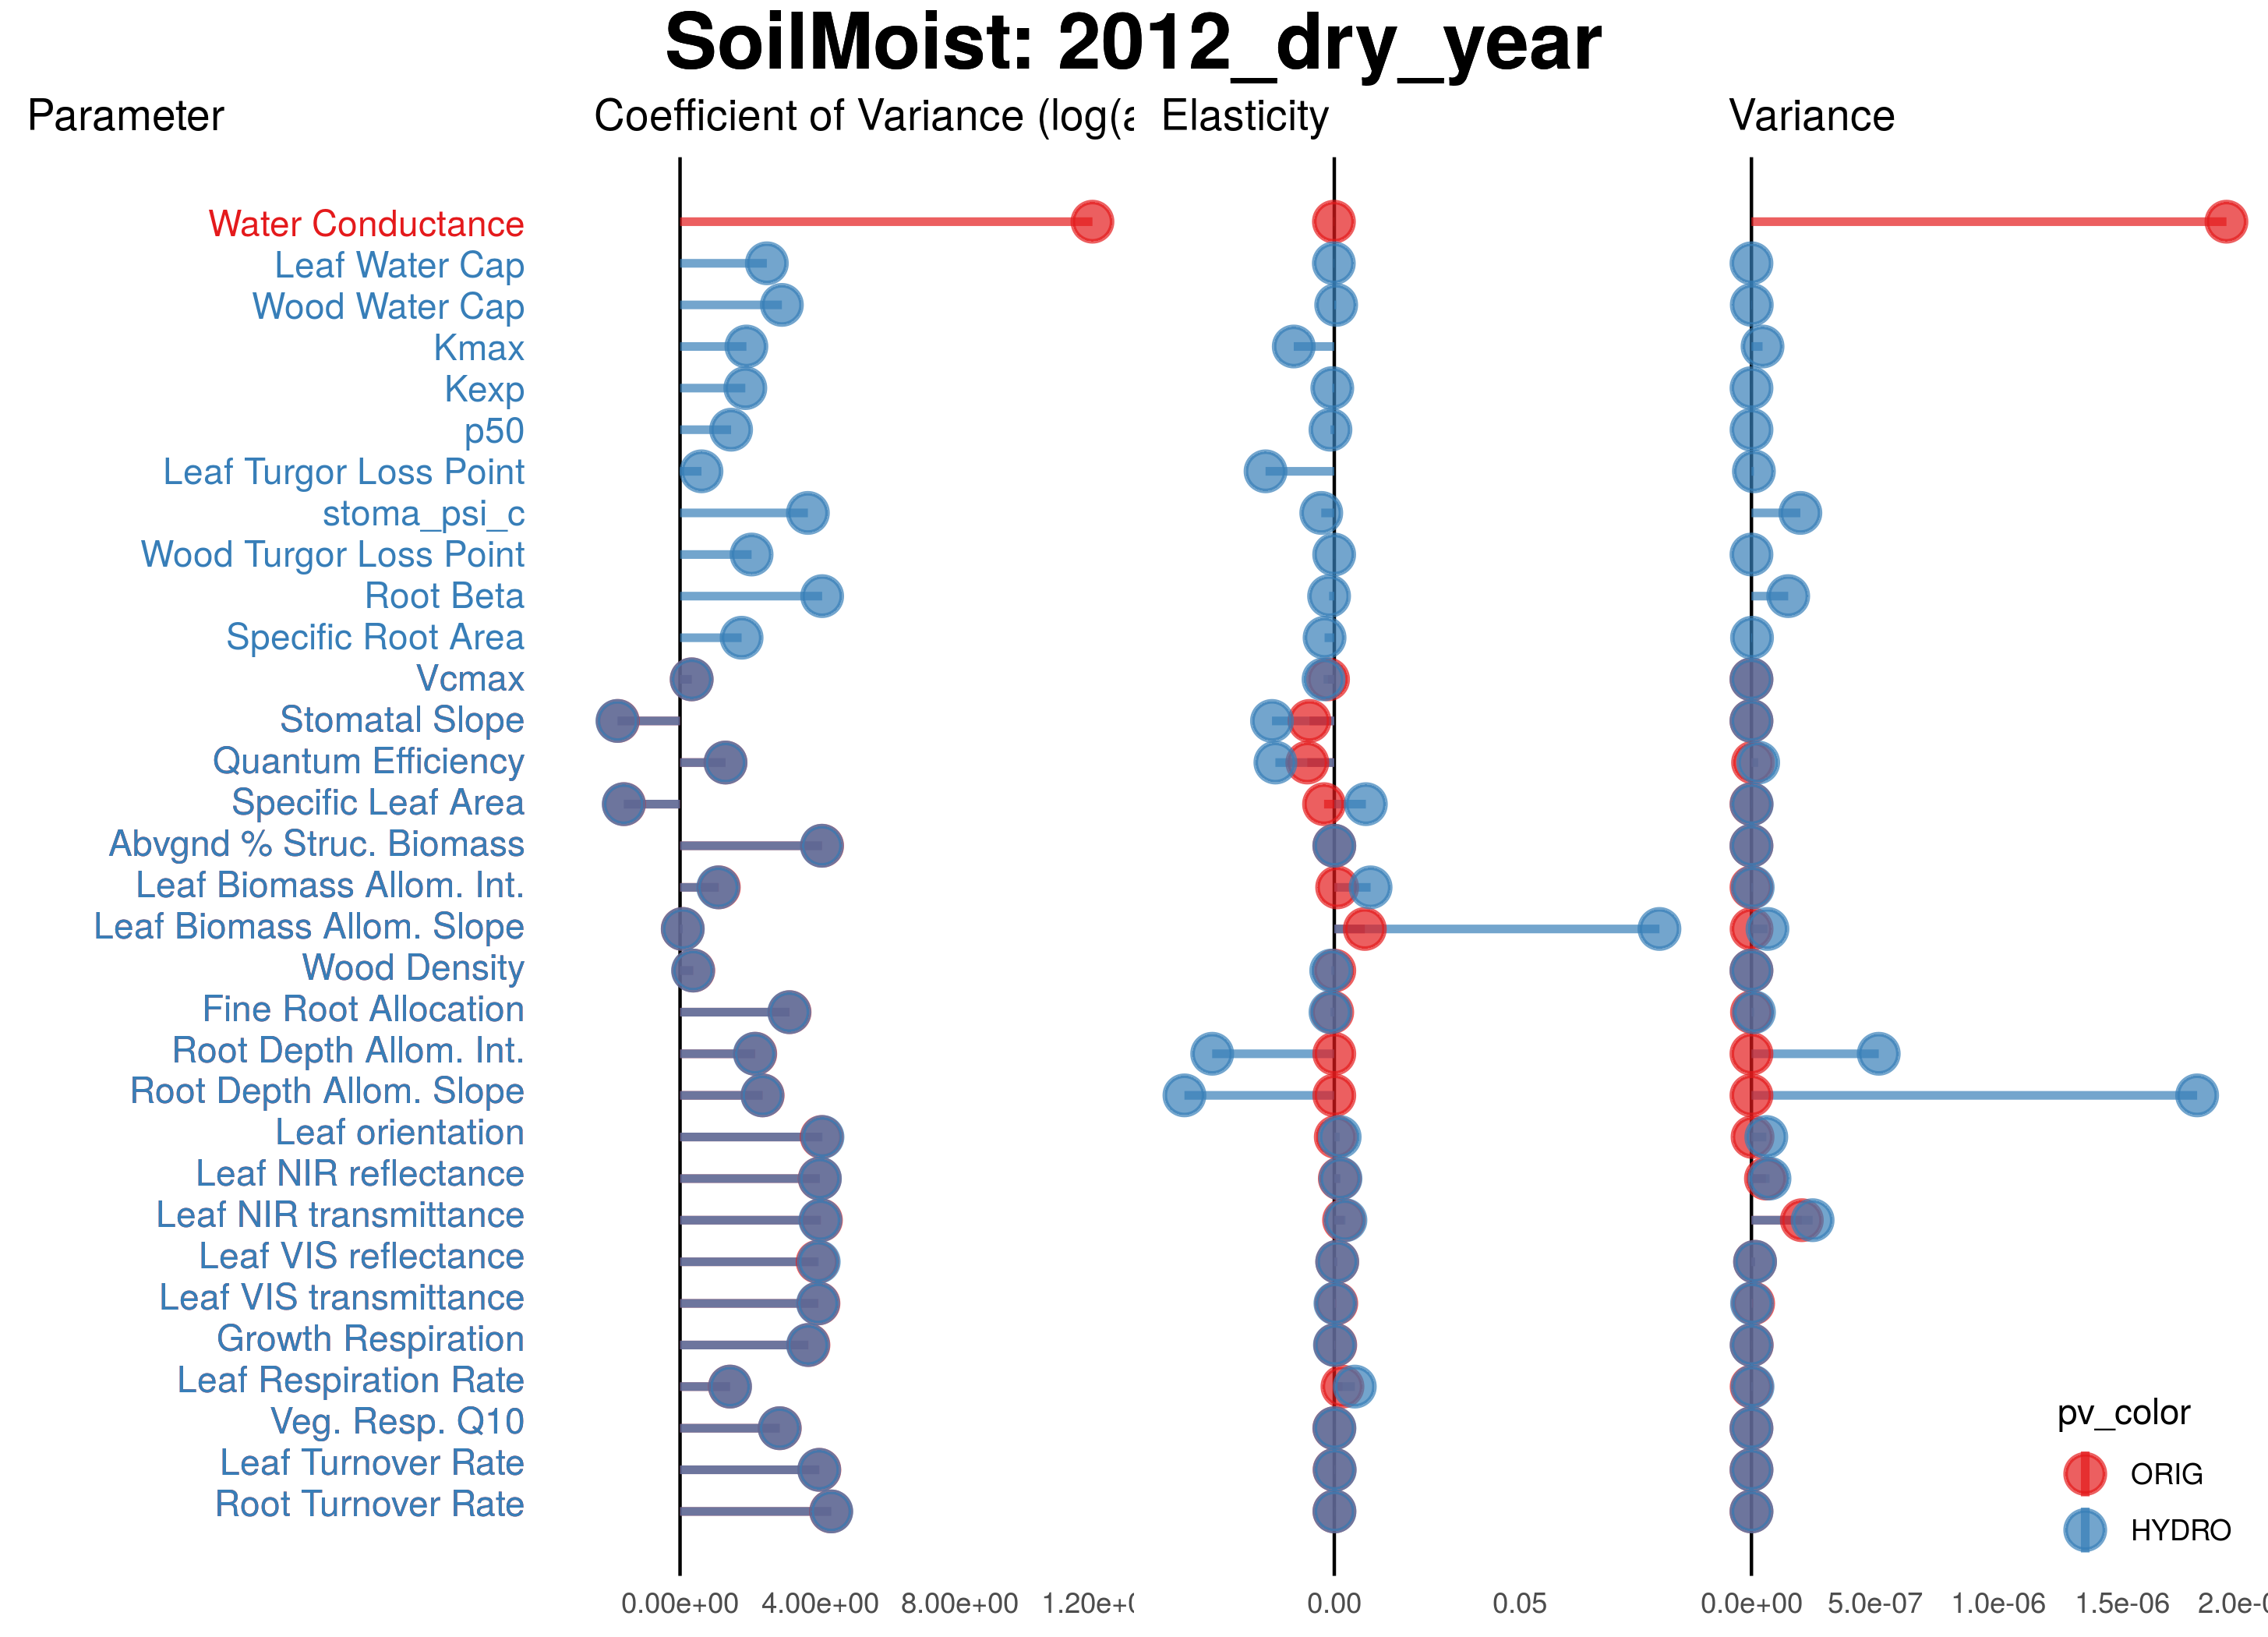
\includegraphics[width=.8\textwidth]{Hydro_Paper_LaTeX/Hydro_Paper_Figures/VDC_SoilMoist_dry.png}
    \caption[Soil Moisture Variance Decomposition]{Variance Decomposition for Soil Moisture Under Dry Conditions, Comparing ED2 and ED2-Hydro}
    \label{fig:constraint_var}
\end{figure}
\begin{figure}[h]
    \centering
    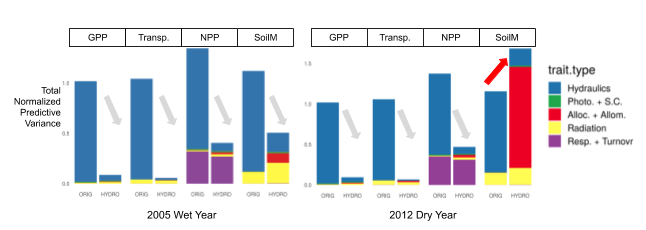
\includegraphics[width=.95\textwidth]{Hydro_Paper_LaTeX/Hydro_Paper_Figures/Total_variance.png}
    \caption[Total Variance]{Total Variance wet and dry years}
    \label{fig:total_var}
\end{figure}

% \begin{wrapfigure}{l}{0.25\textwidth}
%     \centering
%     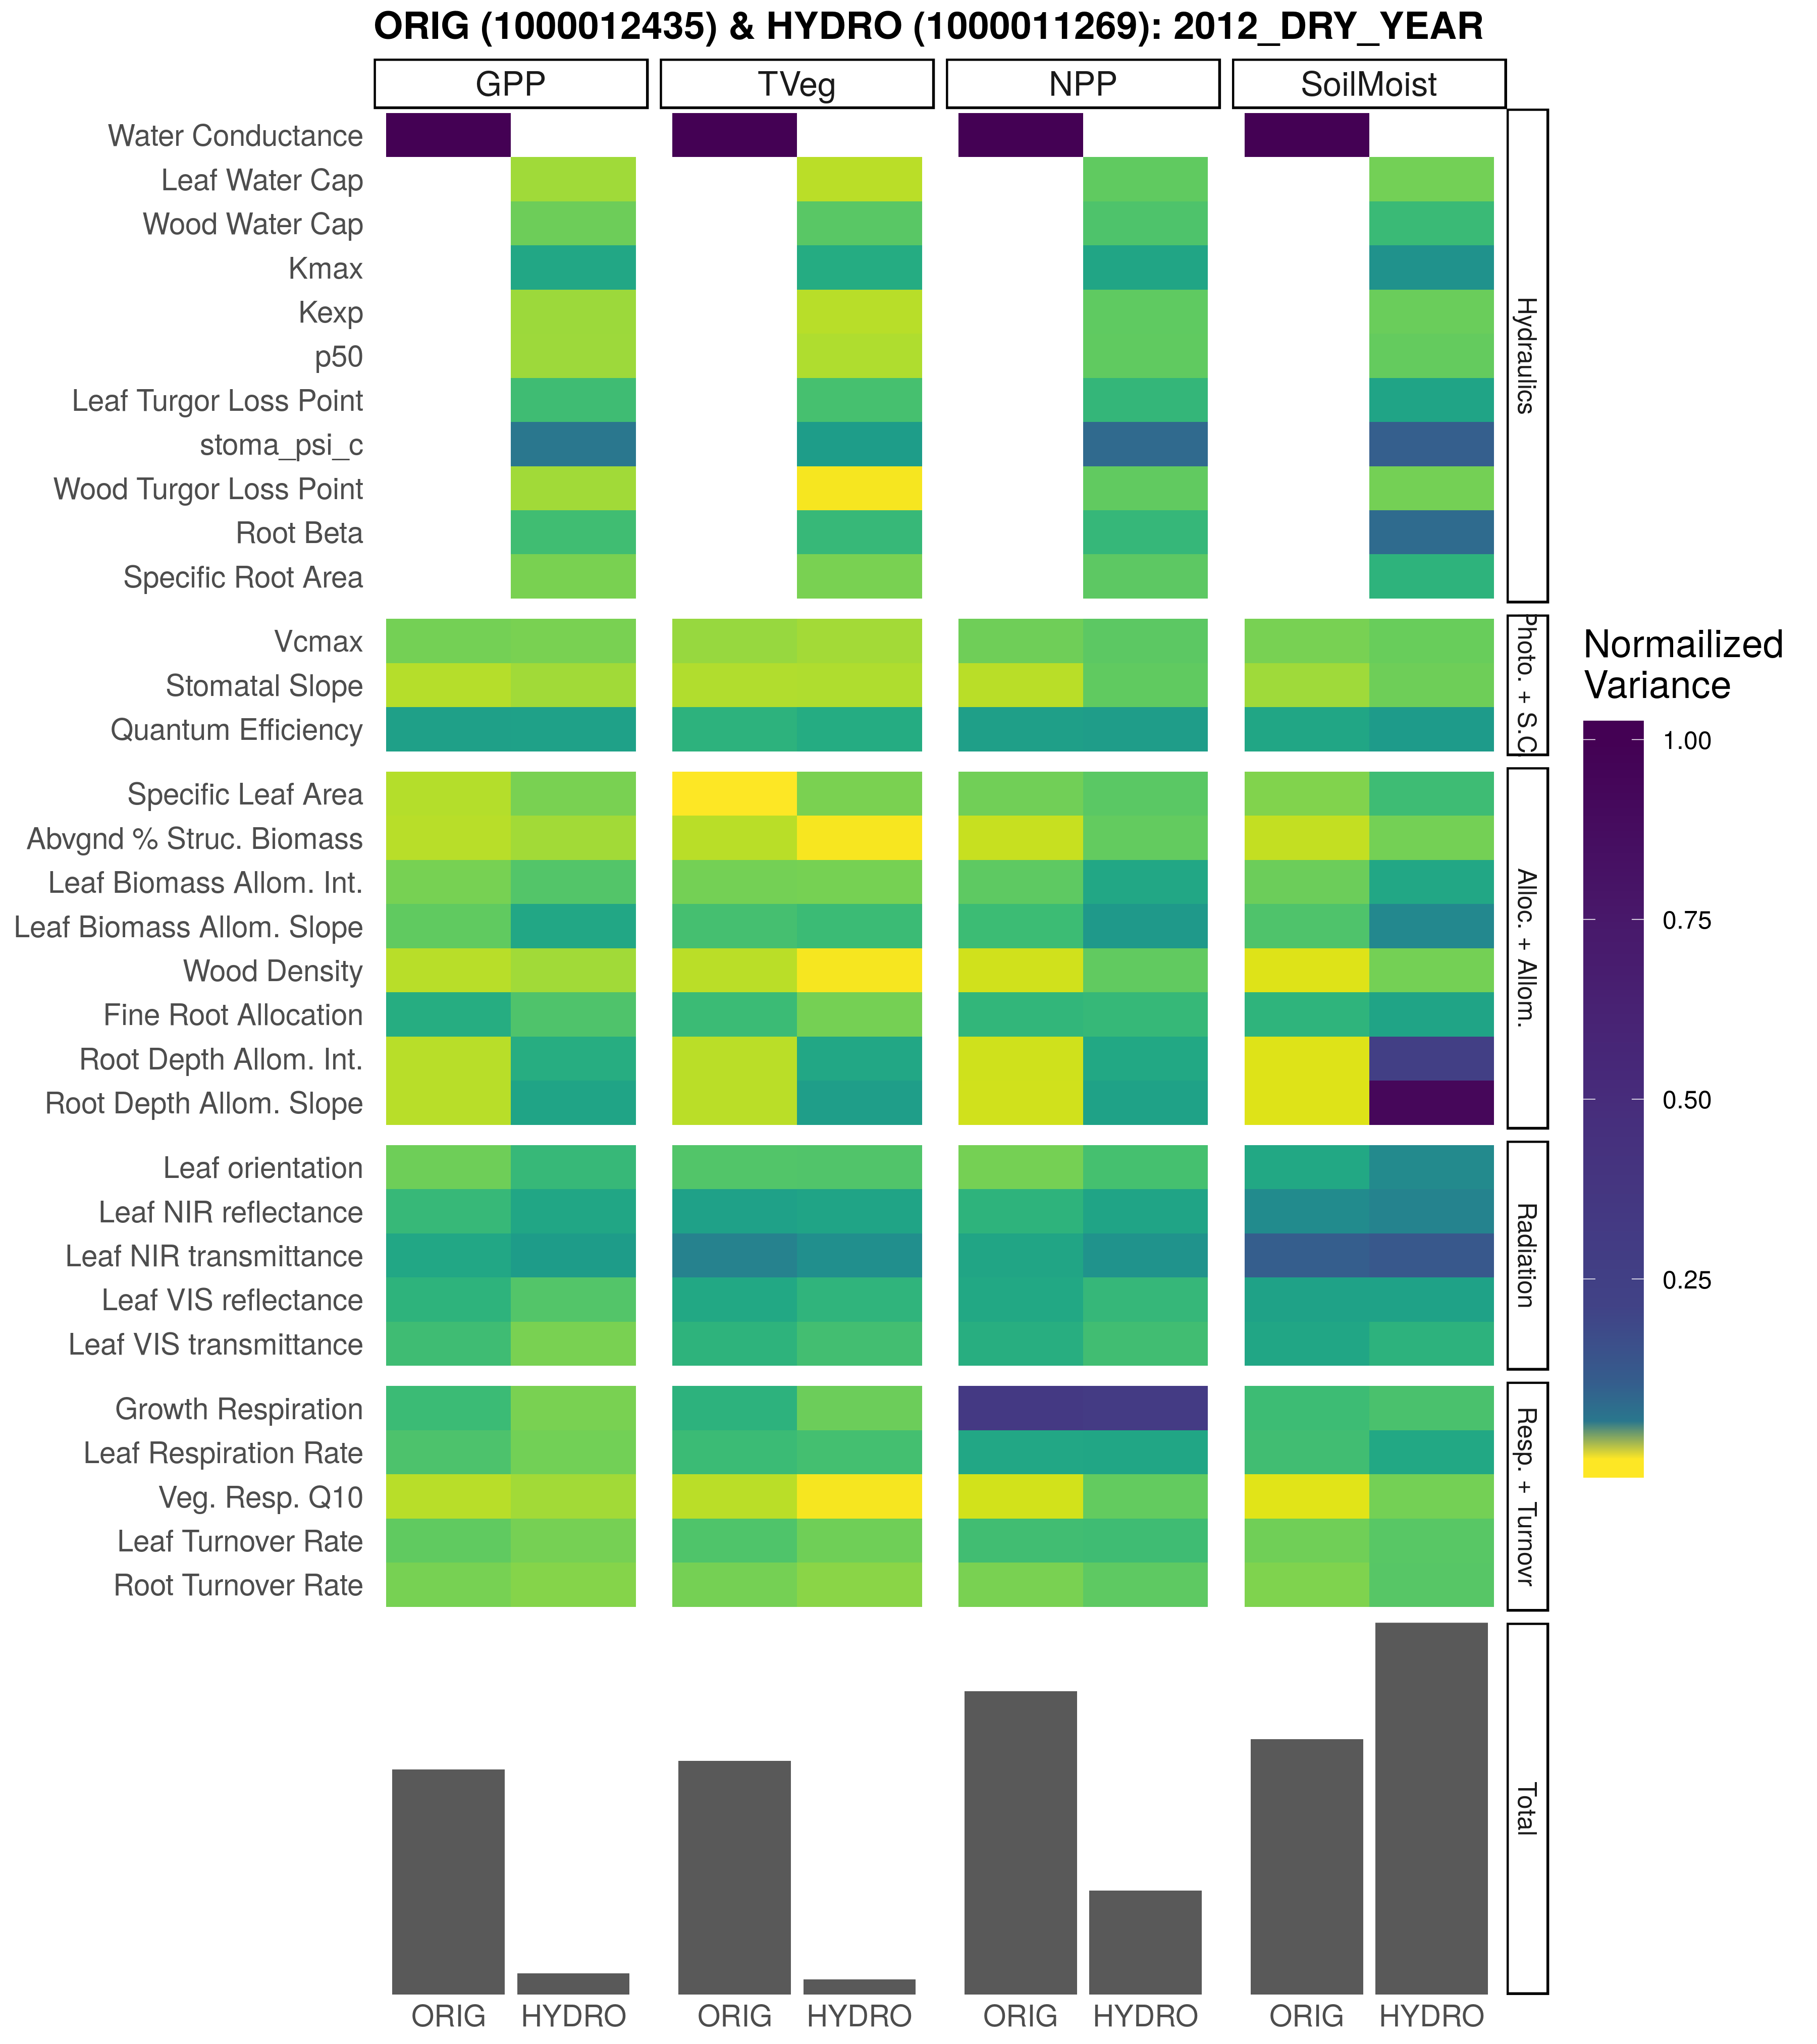
\includegraphics[width=.25\textwidth]{Hydro_Paper_LaTeX/Hydro_Paper_Figures/heatmap_bar_dry_year.png}
%     %\caption{Heatmap of the dry year}
%     %\label{fig:ED_versions}
% \end{wrapfigure}


\begin{figure}[h]
    \centering
    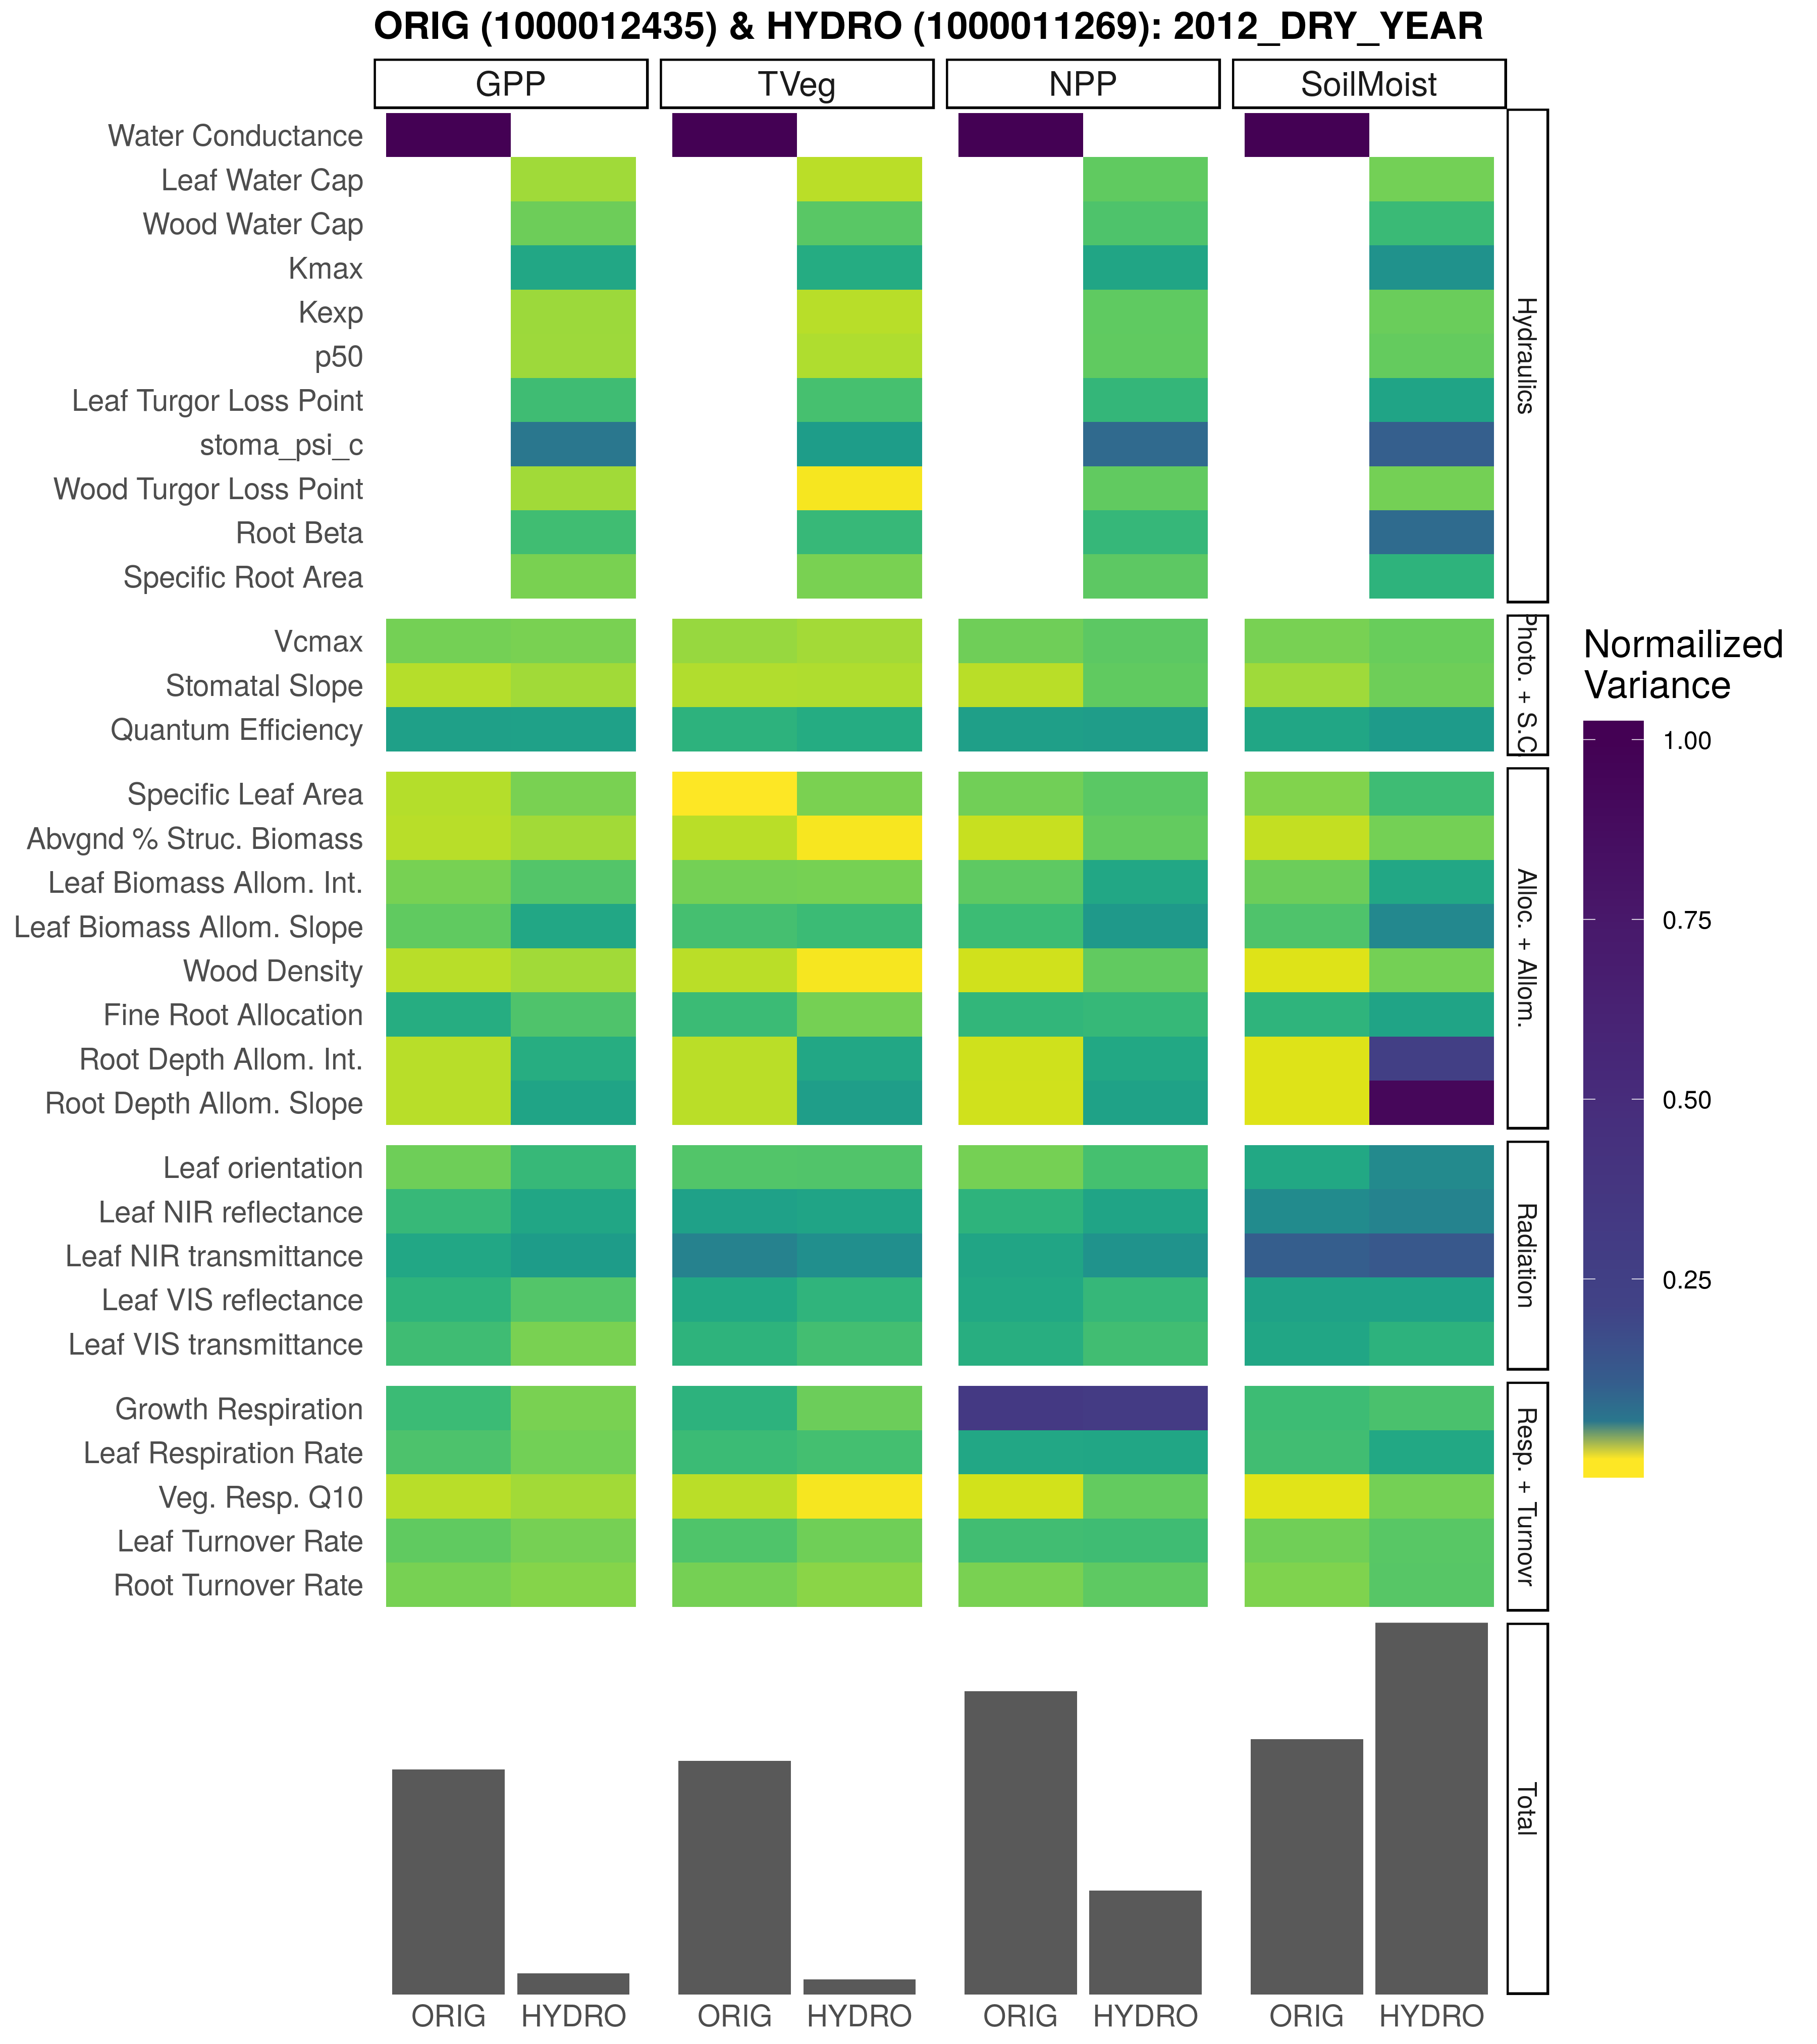
\includegraphics[width=.75\textheight]{Hydro_Paper_LaTeX/Hydro_Paper_Figures/heatmap_bar_dry_year.png}
    \caption[Heatmap of the dry year]{Heat map of the dry year ... }
    \label{fig:heatmap_dry}
\end{figure}
